% This file was created with tikzplotlib v0.10.1.
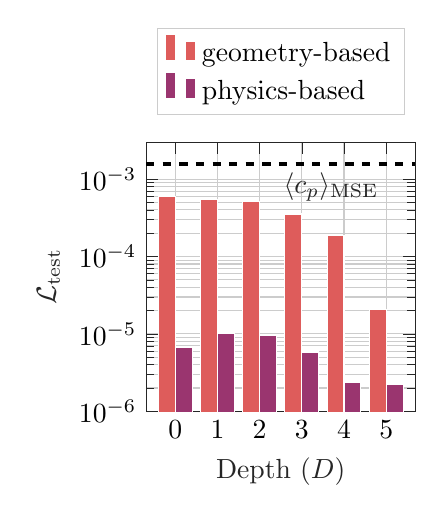
\begin{tikzpicture}

\definecolor{darkslategray38}{RGB}{38,38,38}
\definecolor{indianred2229291}{RGB}{222,92,91}
\definecolor{lightgray204}{RGB}{204,204,204}
\definecolor{mediumvioletred15453111}{RGB}{154,53,111}

\begin{axis}[
width=5cm,
height=5cm,
axis line style={darkslategray38},
legend cell align={left},
legend columns = 1,
legend style={
  fill opacity=1,
  draw opacity=1,
  text opacity=1,
  at={(0.5,1.1)},
  anchor=south,
  draw=lightgray204,
  % column sep = 0.1cm
},
log basis y={10},
tick align=inside,
x grid style={lightgray204},
xlabel=\textcolor{darkslategray38}{Depth (\(\displaystyle D\))},
xmajorgrids,
xmajorticks=true,
xmin=-0.69, xmax=5.69,
% xminorgrids,
xtick style={color=darkslategray38},
xtick={0,1,2,3,4,5},
xticklabels={
  \(\displaystyle {0}\),
  \(\displaystyle {1}\),
  \(\displaystyle {2}\),
  \(\displaystyle {3}\),
  \(\displaystyle {4}\),
  \(\displaystyle {5}\)
},
y grid style={lightgray204},
ylabel=\textcolor{darkslategray38}{\(\displaystyle \mathcal{L}_{\mathrm{test}}\)},
ymajorgrids,
ymajorticks=true,
% ymin=1.59801652953767e-06, ymax=0.003,
yminorgrids,
% ymode=log,
% ytick style={color=darkslategray38}
ymin=1e-06, ymax=0.003,
    ymode=log,
    ytick style={color=darkslategray38},
    % ytick={1e-06,1e-05,0.0001,0.001},
    % yticklabels={
    %   \(\displaystyle {10^{-6}}\),
    %   \(\displaystyle {10^{-5}}\),
    %   \(\displaystyle {10^{-4}}\),
    %   \(\displaystyle {10^{-3}}\)
    % }
]
\def\epsVal{1e-8}

\draw[draw=white,fill=indianred2229291] (axis cs:-0.4,\epsVal) rectangle (axis cs:0,0.000597328355);
\addlegendimage{ybar,ybar legend,draw=white,fill=indianred2229291, legend image post style={xscale=1.2,yscale=1.2}}
% \addlegendentry{GBF}
\addlegendentry{geometry-based}

\draw[draw=white,fill=indianred2229291] (axis cs:0.6,\epsVal) rectangle (axis cs:1,0.000545040821);
\draw[draw=white,fill=indianred2229291] (axis cs:1.6,\epsVal) rectangle (axis cs:2,0.000514299027);
\draw[draw=white,fill=indianred2229291] (axis cs:2.6,\epsVal) rectangle (axis cs:3,0.000353918178);
\draw[draw=white,fill=indianred2229291] (axis cs:3.6,\epsVal) rectangle (axis cs:4,0.000186683203);
\draw[draw=white,fill=indianred2229291] (axis cs:4.6,\epsVal) rectangle (axis cs:5,2.07822668e-05);
\draw[draw=white,fill=mediumvioletred15453111] (axis cs:-2.77555756156289e-17,\epsVal) rectangle (axis cs:0.4,6.62764569e-06);
\addlegendimage{ybar,ybar legend,draw=white,fill=mediumvioletred15453111, legend image post style={xscale=1.2,yscale=1.2}}
% \addlegendentry{PBF}
\addlegendentry{physics-based}

\draw[draw=white,fill=mediumvioletred15453111] (axis cs:1,\epsVal) rectangle (axis cs:1.4,1.02298527e-05);
\draw[draw=white,fill=mediumvioletred15453111] (axis cs:2,\epsVal) rectangle (axis cs:2.4,9.47453918e-06);
\draw[draw=white,fill=mediumvioletred15453111] (axis cs:3,\epsVal) rectangle (axis cs:3.4,5.85003636e-06);
\draw[draw=white,fill=mediumvioletred15453111] (axis cs:4,\epsVal) rectangle (axis cs:4.4,2.36108303e-06);
\draw[draw=white,fill=mediumvioletred15453111] (axis cs:5,\epsVal) rectangle (axis cs:5.4,2.21809773e-06);
\addplot [line width = 1.5pt, dashed, black]
table {%
-0.69 0.00156303530093282
5.69 0.00156303530093282
};

\draw (axis cs:2.34,0.0008) node[
  scale=1,
  anchor=west,
  text=darkslategray38
]{$ \langle c_p \rangle _ {\mathrm{MSE}}$};
\end{axis}

\end{tikzpicture}
